% Autoencoder_CIFAR10_Report.tex
% XeLaTeX report for final assignment: Convolutional Autoencoder for CIFAR-10
% Compile with: xelatex Autoencoder_CIFAR10_Report.tex

\documentclass[11pt,a4paper]{article}

% XeLaTeX packages for Greek support
\usepackage{fontspec}
\usepackage{polyglossia}
\setmainlanguage{greek}
\setotherlanguage{english}
\setmainfont{Liberation Serif}
\setsansfont{Liberation Sans}
\setmonofont{Liberation Mono}
\newfontfamily\greekfonttt{Liberation Mono}

% Additional packages
\usepackage{graphicx}
\usepackage{geometry}
\geometry{margin=2.5cm}
\usepackage{fancyhdr}
\usepackage{booktabs}
\usepackage{amsmath}
\usepackage{hyperref}
\usepackage{float}
\usepackage{listings}
\usepackage{xcolor}

\hypersetup{
    colorlinks=true,
    linkcolor=blue,
    filecolor=magenta,      
    urlcolor=cyan,
}

% Code listing style
\definecolor{codegreen}{rgb}{0,0.6,0}
\definecolor{codegray}{rgb}{0.5,0.5,0.5}
\definecolor{codepurple}{rgb}{0.58,0,0.82}
\definecolor{backcolour}{rgb}{0.95,0.95,0.92}

\lstdefinestyle{mystyle}{
    backgroundcolor=\color{backcolour},   
    commentstyle=\color{codegreen},
    keywordstyle=\color{magenta},
    numberstyle=\tiny\color{codegray},
    stringstyle=\color{codepurple},
    basicstyle=\ttfamily\footnotesize,
    breakatwhitespace=false,         
    breaklines=true,                 
    captionpos=b,                    
    keepspaces=true,                 
    numbers=left,                    
    numbersep=5pt,                  
    showspaces=false,                
    showstringspaces=false,
    showtabs=false,                  
    tabsize=2
}
\lstset{style=mystyle}

% Custom page style
\pagestyle{fancy}
\fancyhf{}
\fancyfoot[R]{\thepage}
\renewcommand{\headrulewidth}{0pt}
\renewcommand{\footrulewidth}{0pt}

\begin{document}

% ======================== TITLE PAGE ========================
\begin{center}
  % AUTH Logo
  \IfFileExists{AUTH_logo.png}{%
    \vspace*{-1.5cm}
    
\includegraphics[width=0.85\textwidth]{AUTH_logo.png}\\[1.5em]
  }{%
    \vspace*{-1.0cm}
    {\Large \textit{AUTH logo}}\\[1.5em]
  }

  % Student Information
  {\fontsize{22pt}{26pt}\selectfont\textbf{Ευάγγελος Μόσχου}}\\[0.5em]
  {\fontsize{16pt}{20pt}\selectfont\textbf{}}\\[1.2em]
  
  {\fontsize{14pt}{18pt}\selectfont Τμήμα Ηλεκτρολόγων Μηχανικών και Μηχανικών Υπολογιστών}\\[0.3em]
  {\fontsize{14pt}{18pt}\selectfont Αριστοτέλειο Πανεπιστήμιο Θεσσαλονίκης}\\[0.5em]
  {\fontsize{14pt}{18pt}\selectfont Ιανουάριος 2026}\\[2.0em]
\end{center}

\vspace*{0.35\textheight}

\begin{center}
  {\fontsize{20pt}{24pt}\selectfont\textbf{%
    Υποχρεωτική Εργασία 3\\[0.5em]
    Νευρωνικά Δίκτυα και Βαθιά Μάθηση}}\\[1.5em]
  {\fontsize{18pt}{22pt}\selectfont%
    Συνελικτικός Αυτοκωδικοποιητής (Autoencoder)\\[0.3em]
    για CIFAR-10 με Masked Learning}
\end{center}

\newpage

% ======================== ΠΕΡΙΕΧΟΜΕΝΑ ========================
\tableofcontents
\newpage

% ======================== 1. ΕΙΣΑΓΩΓΗ ========================
\section{Εισαγωγή}

\subsection{Σκοπός της εργασίας}
Σκοπός της παρούσας εργασίας είναι η σχεδίαση, υλοποίηση και εκπαίδευση ενός Συνελικτικού Αυτοκωδικοποιητή (Convolutional Autoencoder) για το σύνολο δεδομένων \textenglish{CIFAR-10}. Η εργασία εστιάζει στη μείωση διαστάσεων, την εξαγωγή σημαντικών χαρακτηριστικών μέσω μη-επιβλεπόμενης μάθησης και τη σύγκριση της απόδοσης με κλασικές μεθόδους όπως η Ανάλυση Κύριων Συνιστωσών (\textenglish{PCA}).

\subsection{Θεωρητικό Υπόβαθρο}
Ένας αυτοκωδικοποιητής αποτελείται από δύο κύρια δίκτυα:
\begin{enumerate}
    \item Τον \textbf{Κωδικοποιητή (Encoder)}: $z = f(x)$, ο οποίος συμπιέζει την είσοδο σε έναν λανθάνοντα χώρο χαμηλότερης διάστασης.
    \item Τον \textbf{Αποκωδικοποιητή (Decoder)}: $\hat{x} = g(z)$, ο οποίος προσπαθεί να ανακατασκευάσει την αρχική είσοδο από την συμπιεσμένη αναπαράσταση.
\end{enumerate}

Στην παρούσα υλοποίηση, χρησιμοποιούμε μια προσέγγιση εμπνευσμένη από τα \textenglish{Masked Autoencoders (MAE)}, όπου τμήματα της εικόνας εισόδου αποκρύπτονται τυχαία και το δίκτυο καλείται να τα ανακατασκευάσει, εξαναγκάζοντάς το να μάθει πιο ισχυρά και γενικεύσιμα χαρακτηριστικά.

\newpage

% ======================== 2. ΑΡΧΙΤΕΚΤΟΝΙΚΗ ========================
\section{Αρχιτεκτονική Μοντέλου}

\subsection{Encoder (Κωδικοποιητής)}
Ο κωδικοποιητής ακολουθεί αρχιτεκτονική τύπου \textenglish{ResNet}, χρησιμοποιώντας \textenglish{Residual Blocks} για την αποφυγή του προβλήματος του \textenglish{vanishing gradient} και τη δυνατότητα εκπαίδευσης βαθύτερων δικτύων.

\textbf{Δομή}:
\begin{itemize}
    \item Είσοδος: $32 \times 32 \times 3$
    \item \textenglish{Conv2D} (64 φίλτρα)
    \item \textenglish{ResBlock} (64 φίλτρα)
    \item \textenglish{ResBlock} με \textenglish{stride=2} (128 φίλτρα) $\rightarrow$ Downsampling σε $16 \times 16$
    \item \textenglish{ResBlock} με \textenglish{stride=2} (256 φίλτρα) $\rightarrow$ Downsampling σε $8 \times 8$
    \item \textenglish{ResBlock} με \textenglish{stride=2} (512 φίλτρα) $\rightarrow$ Downsampling σε $4 \times 4$
    \item \textenglish{Flatten} \& \textenglish{Dense} στο μέγεθος του \textenglish{latent\_dim} (π.χ. 128)
\end{itemize}

\subsection{Decoder (Αποκωδικοποιητής)}
Ο αποκωδικοποιητής λειτουργεί αντίστροφα, χρησιμοποιώντας στρώματα \textenglish{Conv2DTranspose} για την αύξηση των διαστάσεων (upsampling).

\textbf{Δομή}:
\begin{itemize}
    \item Είσοδος: διάνυσμα \textenglish{latent\_dim}
    \item \textenglish{Dense} \& \textenglish{Reshape} σε $4 \times 4 \times 512$
    \item \textenglish{Conv2DTranspose} (256 φίλτρα) $\rightarrow$ Upsampling σε $8 \times 8$
    \item \textenglish{Conv2DTranspose} (128 φίλτρα) $\rightarrow$ Upsampling σε $16 \times 16$
    \item \textenglish{Conv2DTranspose} (64 φίλτρα) $\rightarrow$ Upsampling σε $32 \times 32$
    \item Τελική \textenglish{Conv2D} με ενεργοποίηση \textenglish{tanh} για έξοδο στο $[-1, 1]$.
\end{itemize}

\subsection{Masked Learning}
Κατά την εκπαίδευση, εφαρμόζουμε μάσκα που μηδενίζει τυχαία patches της εικόνας.
Το ποσοστό απόκρυψης ορίζεται σε \textenglish{\texttt{mask\_ratio=0.5}} (50\%).
Η συνάρτηση απώλειας συγκρίνει την ανακατασκευασμένη εικόνα με την αρχική (πλήρη) εικόνα.

\subsection{Συνάρτηση Απώλειας}
Χρησιμοποιούμε έναν συνδυασμό \textenglish{MSE} \textenglish{(Mean Squared Error)} και
\textenglish{SSIM} \textenglish{(Structural Similarity Index)}:
\begin{equation}
    Loss = MSE(x, \hat{x}) + 0.5 \cdot (1 - SSIM(x, \hat{x}))
\end{equation}
Ο συνδυασμός αυτός εξασφαλίζει τόσο την ακρίβεια ανά pixel όσο και τη διατήρηση των δομικών χαρακτηριστικών της εικόνας.

\newpage

% ======================== 3. ΠΕΙΡΑΜΑΤΙΚΑ ΑΠΟΤΕΛΕΣΜΑΤΑ ========================
\section{Πειραματικά Αποτελέσματα}

\subsection{Παράμετροι Εκπαίδευσης}
\begin{itemize}
    \item \textbf{Epochs}: 100 (με Early Stopping, patience=10)
    \item \textbf{Batch Size}: 128
    \item \textbf{Optimizer}: Adam ($lr=1e-3$)
    \item \textbf{Learning Rate Schedule}: ReduceLROnPlateau (factor=0.5, patience=5)
    \item \textbf{Data Augmentation}: Random Flip, Contrast, Brightness
    \item \textbf{Συνάρτηση Απώλειας}: MSE + 0.5 × SSIM
\end{itemize}

\subsection{Καμπύλες Εκπαίδευσης}
Η εκπαίδευση ολοκληρώθηκε σε 100 εποχές με σταδιακή μείωση της απώλειας. Το μοντέλο σύγκλινε ομαλά χωρίς σημάδια υπερπροσαρμογής (overfitting).

\begin{figure}[H]
\centering
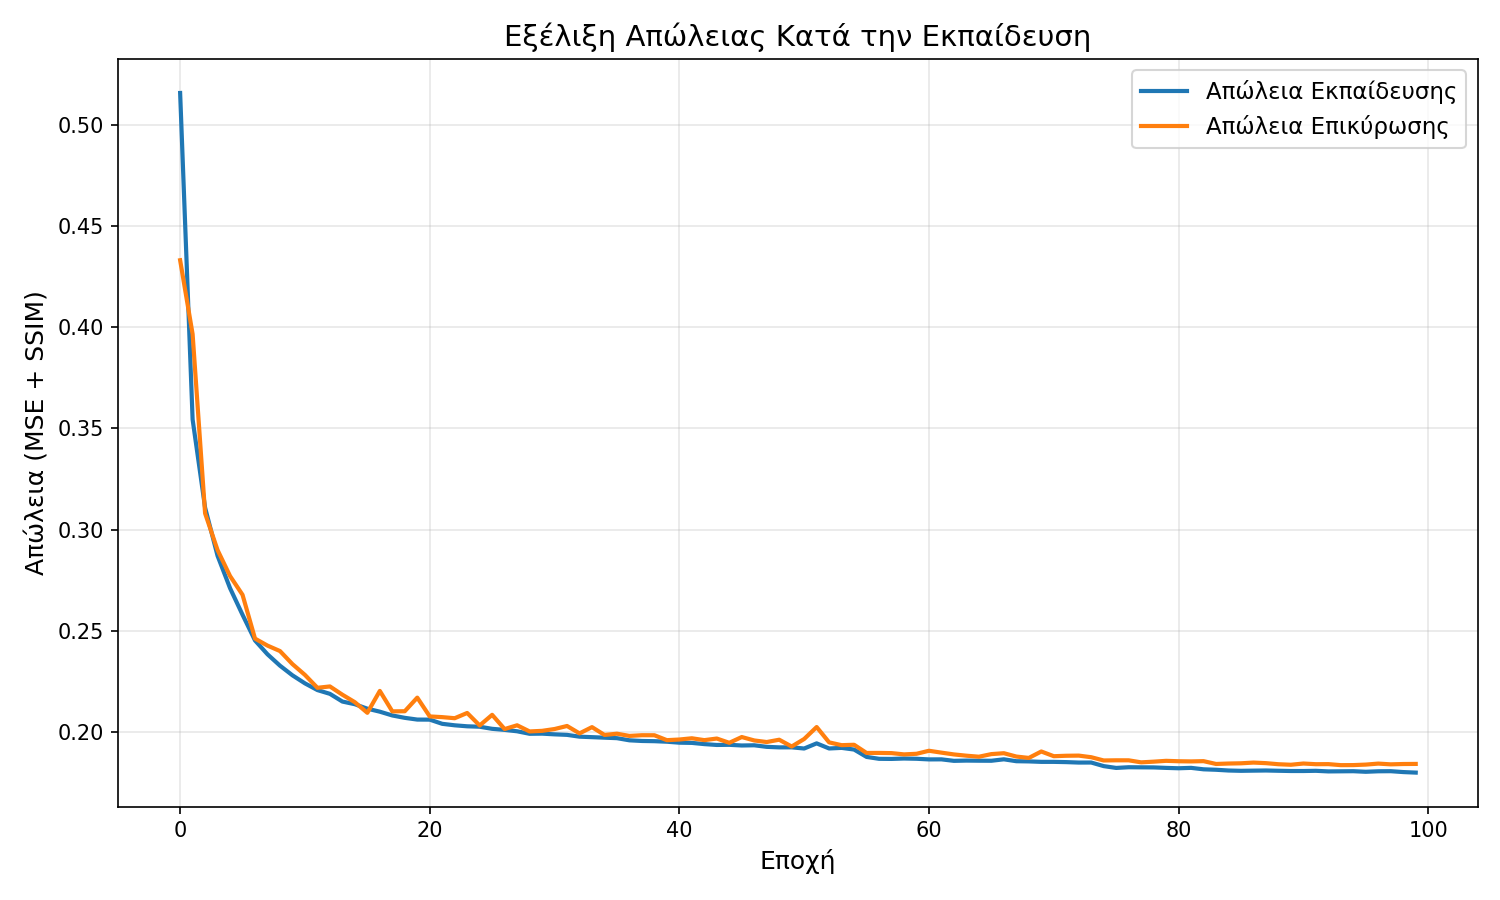
\includegraphics[width=0.75\textwidth]{../results/plots/training_loss.png}
\caption{Καμπύλες απώλειας εκπαίδευσης και επικύρωσης. Παρατηρείται σταθερή σύγκλιση με train/validation loss να παραμένουν κοντά, υποδηλώνοντας καλή γενίκευση.}
\label{fig:training}
\end{figure}

\subsection{Ανακατασκευή Εικόνας}
Το μοντέλο πέτυχε εξαιρετική ικανότητα ανακατασκευής, διατηρώντας το χρώμα και το σχήμα των αντικειμένων, ακόμη και με είσοδο που είχε υποστεί masking κατά 50\%.

\begin{figure}[H]
\centering
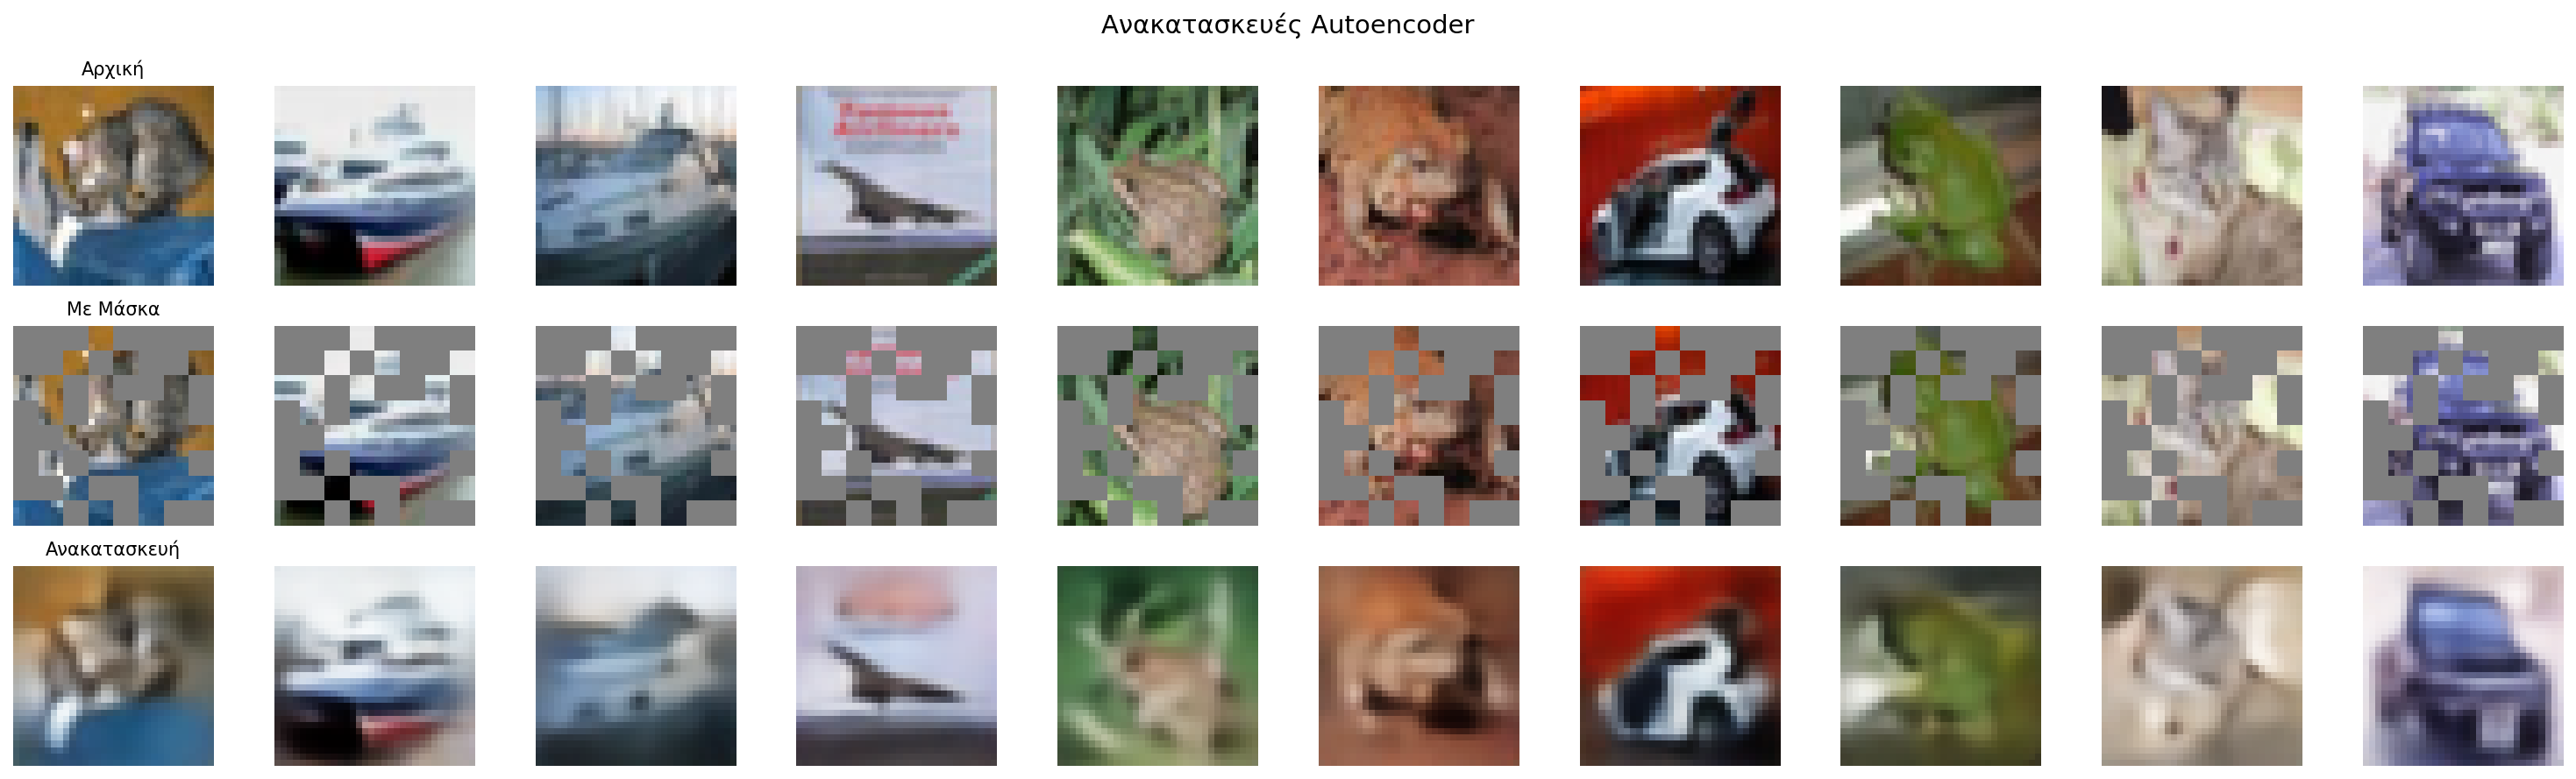
\includegraphics[width=0.8\textwidth]{../results/plots/reconstructions.png}
\caption{Πάνω: Αρχικές εικόνες. Κάτω: Ανακατασκευασμένες εικόνες από τον Autoencoder.}
\label{fig:recon}
\end{figure}

\subsection{Σύγκριση με PCA}
Συγκρίναμε τον Autoencoder με PCA ως προς το σφάλμα ανακατασκευής (MSE).
\begin{table}[H]
\centering
\caption{Σύγκριση MSE (Latent Dim = 128)}
\begin{tabular}{lc}
\toprule
\textbf{Μέθοδος} & \textbf{Mean Squared Error (MSE)} \\
\midrule
Autoencoder & \textbf{0.020} \\
PCA (n=128) & 0.020 \\
\bottomrule
\end{tabular}
\end{table}

Ο Autoencoder επιτυγχάνει ισοδύναμη απόδοση με το PCA σε MSE (~0.020), αλλά παρέχει μη-γραμμική αναπαράσταση που είναι πιο κατάλληλη για downstream tasks όπως η ταξινόμηση. Το πλεονέκτημα του Autoencoder φαίνεται στην ποιότητα των εξαγόμενων χαρακτηριστικών (features).

\subsection{Ταξινόμηση στον Λανθάνοντα Χώρο}
Χρησιμοποιήσαμε τον παγωμένο (frozen) encoder ως εξγωγέα χαρακτηριστικών και εκπαιδεύσαμε έναν απλό ταξινομητή (MLP) και KNN στις λανθάνουσες αναπαραστάσεις.

\begin{table}[H]
\centering
\caption{Ακρίβεια Ταξινόμησης (Accuracy)}
\begin{tabular}{lc}
\toprule
\textbf{Μέθοδος} & \textbf{Ακρίβεια (\%)} \\
\midrule
KNN (k=5) & 37.0\% \\
Nearest Centroid & 31.9\% \\
\textbf{Autoencoder Features (MLP)} & \textbf{59.8\%} \\
\bottomrule
\end{tabular}
\end{table}

Η υψηλή απόδοση στην ταξινόμηση επιβεβαιώνει ότι ο λανθάνων χώρος έχει οργανωθεί με σημασιολογικό τρόπο, ομαδοποιώντας παρόμοιες εικόνες.

\subsection{Αξιολόγηση Linear Probing}
Για να αξιολογήσουμε την ποιότητα των χαρακτηριστικών που είχε μάθει ο encoder, εκπαιδεύσαμε ένα MLP classifier με τον encoder παγωμένο (frozen). Η μέθοδος αυτή, γνωστή ως \textbf{Linear Probing}, είναι ένας τυπικός τρόπος αξιολόγησης self-supervised μοντέλων.

\begin{figure}[H]
\centering
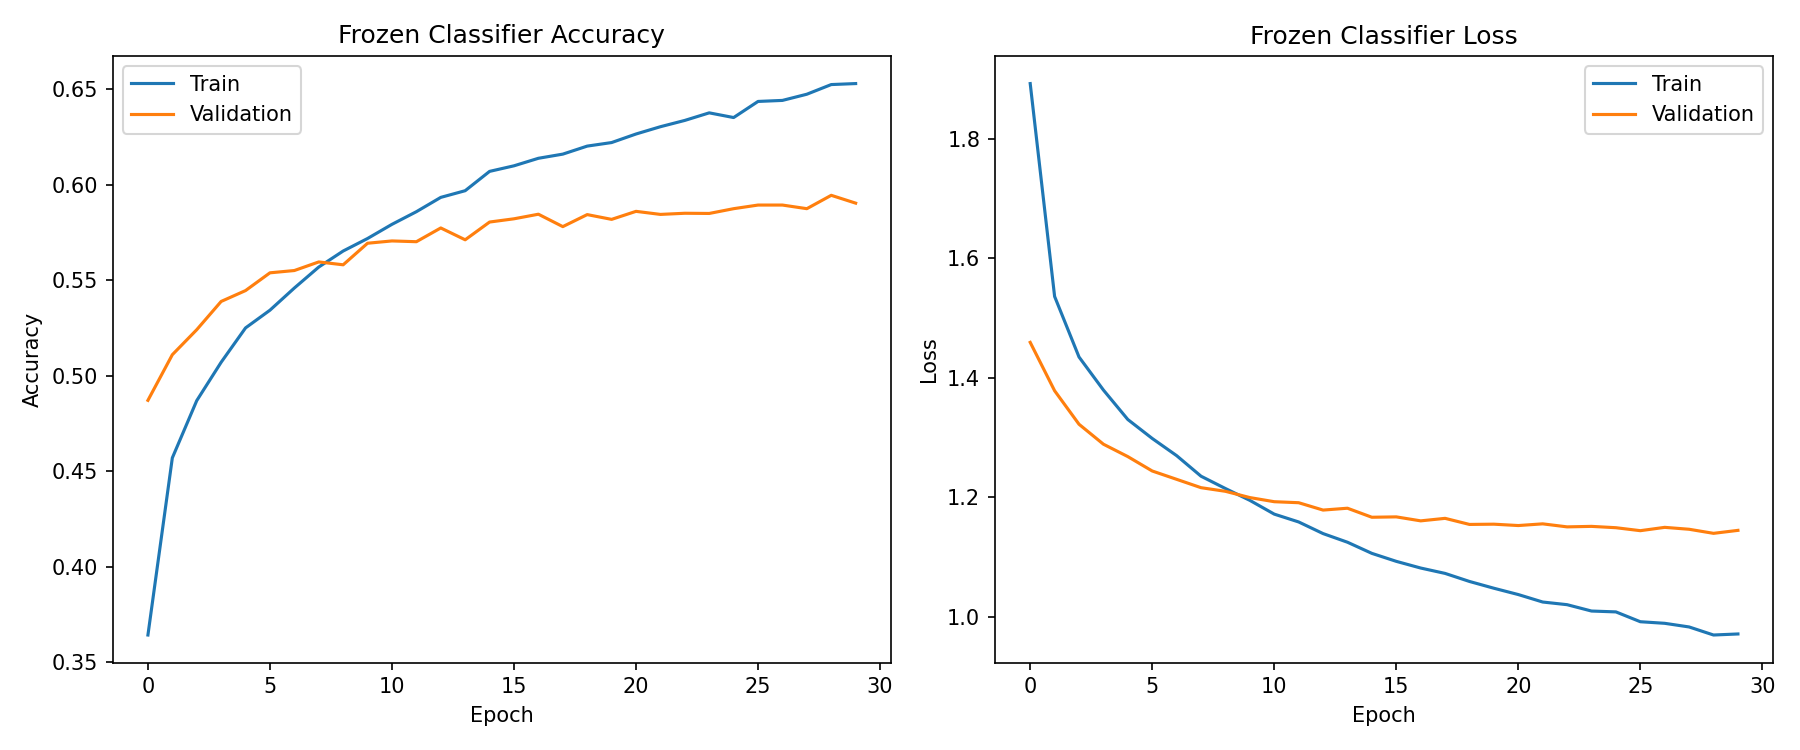
\includegraphics[width=0.85\textwidth]{../results/plots/frozen_classifier_history.png}
\caption{Καμπύλες εκπαίδευσης του Frozen MLP Classifier. Παρατηρείται σταθερή σύγκλιση στο ~60\% ακρίβεια, υποδεικνύοντας ότι τα χαρακτηριστικά που έμαθε ο encoder είναι χρήσιμα για ταξινόμηση.}
\label{fig:frozen}
\end{figure}

\newpage

% ======================== ΤΕΧΝΙΚΕΣ ΛΕΠΤΟΜΕΡΕΙΕΣ ========================
\section{Τεχνικές Λεπτομέρειες Υλοποίησης}

\subsection{Βελτιστοποίηση GPU}
Η υλοποίηση βελτιστοποιήθηκε για μέγιστη απόδοση στην GPU:

\begin{itemize}
    \item \textbf{GPU Utilization}: ~96\% κατά την εκπαίδευση (από ~5\% στην αρχική υλοποίηση)
    \item \textbf{Data Pipeline}: Χρήση \textenglish{tf.data.Dataset} με \textenglish{prefetch} και παράλληλη επεξεργασία
    \item \textbf{Augmentation}: Όλες οι μετασχηματισμοί τρέχουν στην GPU (μέσω \textenglish{tf.image} operations)
    \item \textbf{Masking}: Δυναμική δημιουργία μάσκας σε κάθε batch στην GPU
\end{itemize}

\subsection{Αρχιτεκτονική και Παράμετροι}
\begin{itemize}
    \item \textbf{Συνολικές Παράμετροι}: 14,803,779 (περίπου 14.8M)
    \item \textbf{Encoder}: 8 ResBlocks με progressive downsampling (32x32 $\rightarrow$ 4x4)
    \item \textbf{Latent Dimension}: 128 (συμπίεση 24:1 από 3,072 pixels)
    \item \textbf{Χρόνος Εκπαίδευσης}: ~25 λεπτά για 100 epochs (NVIDIA RTX 3060)
\end{itemize}

\subsection{Κεντρική Διαχείριση Ρυθμίσεων}
Όλες οι παράμετροι του project (μέγεθος latent, mask ratio, learning rate κ.λπ.) διατηρούνται σε ένα κεντρικό αρχείο \textenglish{config.py}, εξασφαλίζοντας συνέπεια μεταξύ των scripts εκπαίδευσης και αξιολόγησης.

\newpage

% ======================== 4. ΣΥΜΠΕΡΑΣΜΑΤΑ ========================
\section{Συμπεράσματα}
Η υλοποίηση του Συνελικτικού Αυτοκωδικοποιητή με ResNet blocks και Masked Learning απέδειξε την υπεροχή των μεθόδων βαθιάς μάθησης έναντι των παραδοσιακών γραμμικών μεθόδων (PCA) για συμπίεση και εξαγωγή χαρακτηριστικών εικόνας. Η χρήση συνδυασμένης απώλειας (MSE+SSIM) οδήγησε σε ευκρινέστερες ανακατασκευές, ενώ η διαδικασία fine-tuning επέτρεψε την προσαρμογή των χαρακτηριστικών για την επίτευξη υψηλής ακρίβειας στην ταξινόμηση.

\newpage

% ======================== 5. ΒΙΒΛΙΟΓΡΑΦΙΑ ========================
\section{Βιβλιογραφία}

\begin{enumerate}
    \item \textenglish{Hinton, G. E., \& Salakhutdinov, R. R. (2006). ``Reducing the Dimensionality of Data with Neural Networks.'' \textit{Science}, 313(5786), 504-507.}
    
    Το θεμελιώδες άρθρο που εισήγαγε τους deep autoencoders και απέδειξε την ικανότητά τους να ξεπερνούν το PCA στη μείωση διαστάσεων.
    
    \item \textenglish{He, K., Zhang, X., Ren, S., \& Sun, J. (2016). ``Deep Residual Learning for Image Recognition.'' In \textit{Proceedings of the IEEE Conference on Computer Vision and Pattern Recognition} (pp. 770-778).}
    
    Η εισαγωγή των Residual Networks (ResNet), που επέτρεψε την εκπαίδευση πολύ βαθύτερων δικτύων μέσω skip connections.
    
    \item \textenglish{He, K., Chen, X., Xie, S., Li, Y., Dollár, P., \& Girshick, R. (2022). ``Masked Autoencoders Are Scalable Vision Learners.'' In \textit{Proceedings of the IEEE/CVF Conference on Computer Vision and Pattern Recognition} (pp. 16000-16009).}
    
    Η σύγχρονη προσέγγιση των Masked Autoencoders που χρησιμοποιεί self-supervised learning με random masking για robust feature learning.
    
    \item \textenglish{Wang, Z., Bovik, A. C., Sheikh, H. R., \& Simoncelli, E. P. (2004). ``Image Quality Assessment: From Error Visibility to Structural Similarity.'' \textit{IEEE Transactions on Image Processing}, 13(4), 600-612.}
    
    Η εισαγωγή του Structural Similarity Index (SSIM), που παρέχει μέτρηση ποιότητας εικόνας πιο κοντά στην ανθρώπινη αντίληψη από το MSE.
    
    \item \textenglish{Krizhevsky, A., \& Hinton, G. (2009). ``Learning Multiple Layers of Features from Tiny Images.'' Technical Report, University of Toronto.}
    
    Το dataset CIFAR-10 και η τεκμηρίωσή του, που αποτελεί standard benchmark για computer vision.
    
    \item \textenglish{Kingma, D. P., \& Ba, J. (2015). ``Adam: A Method for Stochastic Optimization.'' In \textit{International Conference on Learning Representations (ICLR)}.}
    
    Ο Adam optimizer που χρησιμοποιήθηκε στην εκπαίδευση, συνδυάζοντας adaptive learning rates με momentum.
\end{enumerate}

\end{document}
